\documentclass{beamer}
\usepackage{Presentacion}

\title[Detección de Deadlocks en Rust]{Detección de Deadlocks en Rust \\ en tiempo de compilación \\ mediante Redes de Petri}
\author{Horacio Lisdero Scaffino}
\institute[FIUBA]{Facultad de Ingeniería\\Universidad de Buenos Aires}
\date{19 de febrero del 2023}
% TWEAK THE FONT SIZE
\setbeamerfont{date}{size=\scriptsize}
% ADD LOGO
\logo{
\includegraphics[height=1.3cm]{FIUBA-Logo.png}}

\AtBeginSection[]
{
  \begin{frame}{Agenda}
  \footnotesize
    \tableofcontents[currentsection, currentsubsection]
  \end{frame}
}

\AtBeginSubsection[]
{
  \begin{frame}{Agenda}
  \footnotesize
    \tableofcontents[currentsection, currentsubsection]
  \end{frame}
}

\begin{document}

\begin{frame}
  \titlepage
\end{frame}

% REMOVE THE LOGO FROM NOW ON %
\logo{}

\begin{frame}{Agenda}
  \tableofcontents
\end{frame}

\section{Introducción}

\begin{frame}{Una vista general de la herramienta}
  El traductor es el componente principal.
  El verificador de modelos y el compilador de Rust, \emph{rustc}, son dependencias.

  \begin{figure}
    \centering
    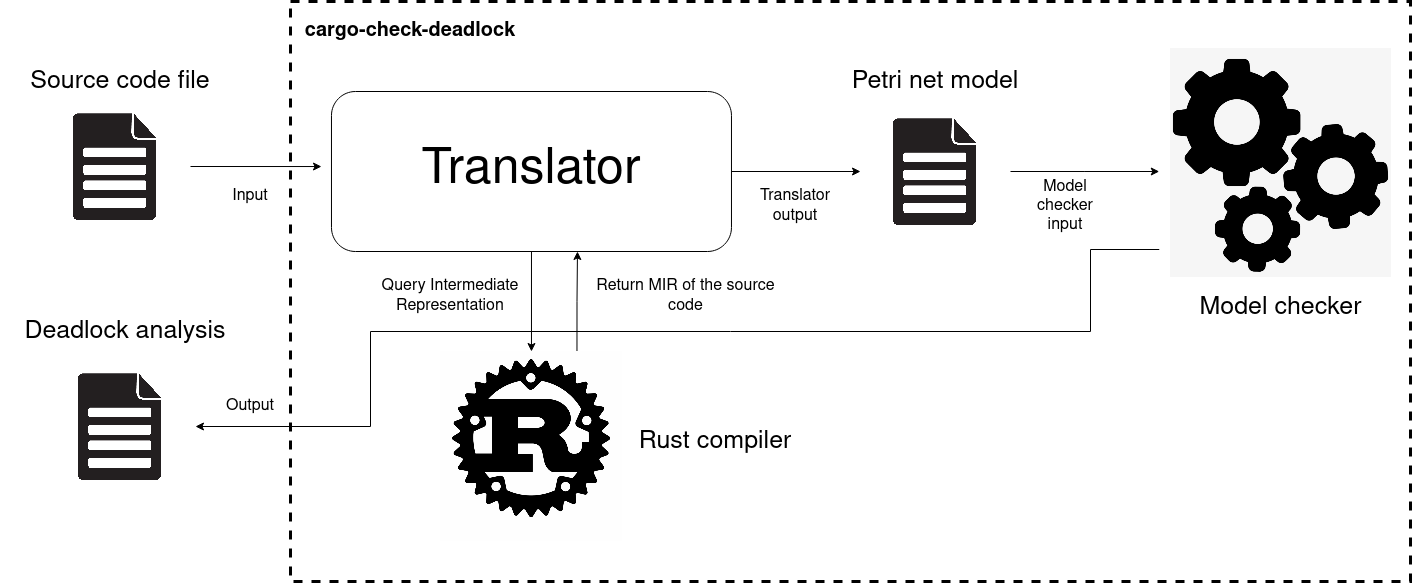
\includegraphics[width=\linewidth]{cargo-check-deadlock-logic-view.png}
  \end{figure}
\end{frame}

\section{Rust}

\subsection{¿Qué es Rust?}

\begin{frame}{¿Qué es Rust?}
  Rust es un lenguaje de programación multiparadigma de uso general que
  busca ofrecer a los desarrolladores una forma segura y eficiente de escribir código de bajo nivel.
  
  \pause
  \vfill

  \begin{itemize}
    \item Uso seguro de la memoria (\emph{Memory safe})
    \item Compilado a código máquina, con un \emph{runtime} mínimo
    \item Expresividad de un lenguaje de alto nivel
    \item Performance de un lenguaje de bajo nivel (similar a C o C++)
  \end{itemize}
\end{frame}

\begin{frame}{Breve línea de tiempo de Rust}
  \begin{description}
    \item [2007] Inicio como un proyecto personal de Graydon Hoare, un programador en Mozilla
    \item [2009] Mozilla comienza a patrocinar oficialmente el proyecto
    \item [2015] Primera versión estable 1.0
    \item [2016] Mozilla lanza Servo, un motor de navegador construido con Rust
    \item [2019] Se estabiliza el soporte de \Rustinline{async}/\Rustinline{await}
    \item [2021] AWS, Huawei, Google, Microsoft y Mozilla crean la Rust Foundation.
    \item [2021] El proyecto Android fomenta el uso de Rust para los componentes del SO por debajo del ART
    \item [2022] El kernel de Linux añade soporte para Rust junto con C
    \item [2023] 8 años consecutivos el lenguaje de programación más querido en la Stack Overflow Developer Survey
  \end{description}
\end{frame}

\begin{frame}{Uso seguro de la memoria}
  Logra un uso seguro de la memoria sin recurrir a un recolector de basura o a un contador de referencias.
  En su lugar, utiliza el concepto de \textbf{ownership} (propiedad) y \textbf{borrowing} (préstamo).

  \vfill
  \pause

  Evita una gran variedad de clases de errores en tiempo de compilación:

  \begin{itemize}
    \item Double free
    \item Use after free
    \item Punteros colgantes (\emph{Dangling pointers})
    \item Condiciones de carrera (\emph{Data races})
    \item Pasaje de variables no seguras entre hilos
  \end{itemize}

  \vfill

  Si se encuentra una violación de las reglas del compilador, el programa simplemente no compilará.
\end{frame}

\subsection{¿Por qué Rust?}

\begin{frame}{Memory safety is critical for reliability and security}
  Empirical investigations have concluded that around 70\% of the vulnerabilities found in
  large C/C++ codebases are due to memory handling errors. This high figure can be observed in
  projects such as:

  \begin{itemize}
    \item Android Open Source Project \cite{memory-bugs-android},
    \item the Bluetooth and media components of Android \cite{memory-bugs-android-media-bluetooth},
    \item the Chromium Projects behind the Chrome web browser \cite{memory-bugs-chrome},
    \item the CSS component of Firefox \cite{memory-bugs-firefox},
    \item iOS and macOS \cite{memory-bugs-ios-macos},
    \item Microsoft products \cite{miller-security-microsoft2019, memory-bugs-microsoft},
    \item Ubuntu \cite{memory-bugs-ubuntu}
  \end{itemize}
\end{frame}

\begin{frame}{Rust adoption is increasing fast}
  \scriptsize
  \begin{itemize}
    \item The Android Open Source Project encourages
          the use of Rust for the SO components
          below the ART \cite{stoep2021}.
    \item The Linux kernel introduces in version 6.1 official tooling
          support for programming components in Rust \cite{corbet2022,desimone2022}.
    \item At Mozilla, the Oxidation project was created in 2015
          to increase the usage of Rust in Firefox and related projects.
          As of March 2023, the lines of code in Rust represent more than
          10\% of the total in Firefox Nightly \cite{mozilla-oxidation}.
    \item At Meta, the use of Rust as a development language server-side
          is approved and encouraged since July 2022 \cite{garcia2022}.
    \item At Cloudflare, a new HTTP proxy in Rust was built from scratch
          to overcome the architectural limitations of NGINX,
          reducing CPU usage by 70\% and memory usage by 67\% \cite{wu2022}.
    \item At Discord, reimplementing a crucial service
          in Rust provided great benefits in performance
          and solved a performance penalty due to the garbage collection in Go \cite{howarth2020}.
    \item At npm Inc., the company behind the npm registry, Rust allowed scaling CPU-bound services
          to more than 1.3 billion downloads per day \cite{rust-npm-case-study}.
    \item A study of Rust-based code found it runs so efficiently
          that it uses half as much electricity as a similar program written in Java,
          a language commonly used at AWS \cite{pereira2017energy}.
  \end{itemize}
\end{frame}

\begin{frame}{The tooling is great and works out of the box}
  \begin{itemize}
    \item \href{https://doc.rust-lang.org/stable/cargo/}{cargo},
          the official package manager: Format, build, test, lint, update, and publish packages.
          \pause
    \item \href{https://doc.rust-lang.org/book/ch11-00-testing.html}{Test harness}
          for unit tests, integration tests, and tests in documentation comments (doctests).
          No third-party libraries needed.
          \pause
    \item An official public registry for Rust packages (called ``crates''): \url{https://crates.io/}.
          \pause
    \item Automatic generation of a static website from the doc comments of the project.
          It is published automatically to \url{https://docs.rs/}.
          \pause
    \item An official linter included with the default installation that catches even more errors
          and spots non-idiomatic code: \href{https://github.com/rust-lang/rust-clippy}{clippy}.
          \pause
    \item Integration with git, GitHub, VSCode, IntelliJ is great and easy to use.
          \pause
    \item A new stable compiler release every 6 weeks \cite{albini2019}.
  \end{itemize}
\end{frame}

\section{Redes de Petri}

\subsection{¿Qué es una red de Petri?}

\begin{frame}{Definición informal}
  A Petri net is a mathematical modeling tool
  used to describe and analyze the behavior of concurrent systems.
  It provides a graphical representation of the system's state and its transitions,
  allowing for visual and formal analysis of complex processes.

  \begin{figure}[!htb]
    \centering
    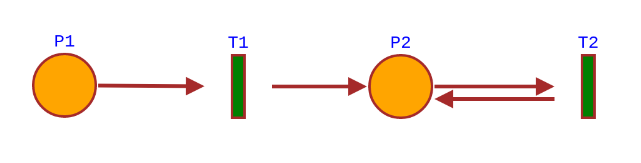
\includegraphics[width=0.8\linewidth]{petri-net-formal-example.png}
  \end{figure}

  \scriptsize
  \begin{itemize}
    \item Places: Represent states in the system (\emph{circles})
    \item Transitions: Represent usually events or actions that occur in the system (\emph{rectangles})
    \item Tokens: Marks inside of places that are created
          and consumed by transitions (\emph{points inside of places})
  \end{itemize}

  \vfill
\end{frame}

\begin{frame}{Mathematical definition}
  A Petri net is a 5-tuple, $ PN = (P, T, F, W, M_{0}) $ where:

  \begin{quote}
    $ P = \{ p_1, p_2, \dots, p_m \} $ is a finite set of places,\\
    $ T = \{ t_1, t_2, \dots, t_n \} $ is a finite set of transitions,\\
    $ F \subseteq (P \times T) \cup (T \times P) $ is a set of arcs (flow relation),\\
    $ W: F \rightarrow \{1, 2, 3, ... \} $ is a weight function for the arcs,\\
    $ M_{0}: P \rightarrow \{0, 1, 2, 3, .... \} $ is the initial marking,\\
    $ P \cap T = \varnothing $ and $ P \cup T \neq \varnothing $
  \end{quote}

  The graph is by definition \emph{bipartite}.
  There can only be edges:
  \begin{itemize}
    \item from places to transitions or
    \item from transitions to places
  \end{itemize}

\end{frame}

\begin{frame}{Transition firing rule}
  \begin{figure}[!htb]
    \centering
    \includesvg[width=0.9\linewidth]{petri-net-transition-example.svg}
  \end{figure}
\end{frame}

\subsection{Ejemplos}

\begin{frame}{Vending machine}
  \scriptsize
  This is a finite-state machine (FSM), a subclass of Petri nets.

  \begin{figure}
    \centering
    \includesvg[width=\linewidth]{state-machine-example.svg}
  \end{figure}
\end{frame}

\begin{frame}{Parallel activities: Fork/Join}
  \scriptsize
  This is a marked graph (MG), a subclass of Petri nets.
  Observe the concurrency between Task 1 and Task 2.
  This cannot be modeled by a single finite-state machine.

  \begin{figure}
    \centering
    \includesvg[width=0.8\linewidth]{parallel-activities-example.svg}
  \end{figure}
\end{frame}

\begin{frame}{Communication protocols: Send with ACK}
  \scriptsize
  A simple protocol in which Process 1 sends messages to Process 2 and
  waits for an acknowledgment to be received before continuing.
  For simplicity, no timeout mechanism was included.

  \begin{figure}
    \centering
    \includesvg[width=0.90\linewidth]{communication-protocols-example.svg}
  \end{figure}
\end{frame}

\begin{frame}{Synchronization control: Readers and writers}
  \scriptsize
  A Petri net system with k processes that either read or write a shared value.

  \begin{itemize}
    \item If one process writes, then no process may read.
    \item If a process is reading, then no process may write.
    \item There can only be zero or one process writing at any given time.
  \end{itemize}

  \begin{figure}
    \centering
    \includesvg[width=0.9\linewidth]{readers-writers-example.svg}
  \end{figure}
\end{frame}

\subsection{¿Por qué usar redes de Petri?}

\begin{frame}{Análisis de alcance}
  Petri nets can be analyzed using formal methods to conclude whether the net can reach
  a deadlock or not. There is a notion of liveness analogous to the one found in computer systems.

  \vfill
  \pause

  Several model checkers are being developed and
  there is even a Model Checking Contest that takes place every year.
  State-of-the-art tools can handle Petri net models
  with more than \textbf{70 000 transitions} and \textbf{one million places}.

  \vfill
  \pause

  Translating source code to a Petri net has been done before for other programming languages
  \cite{kavi2002modeling,moshtaghi2001} and also for Rust \cite{meyer2020, zhang2022deadlocks}.
  The difficulty lies in supporting more synchronization primitives
  than simple mutexes and translating code from real-world applications.
\end{frame}

\section{Traducción}

\begin{frame}{Compilation stages in \emph{rustc}}
  \scriptsize

  \begin{itemize}
    \item Lexing: The source text is turned into a stream of atomic source code units known as tokens.
          \pause
    \item Parsing: The stream of tokens is converted into an \textbf{Abstract Syntax Tree}.
          \pause
    \item High-level Intermediate Representation (HIR):
          \begin{itemize}
            \scriptsize
            \setbeamertemplate{itemize items}[circle]
            \item Desugar loops: \Rustinline[fontsize=\scriptsize]{while} and \Rustinline[fontsize=\scriptsize]{for} to simple \Rustinline[fontsize=\scriptsize]{loop}.
            \item Type inference: The automatic detection of a type of an expression.
            \item Trait solving: Ensuring that each implementation block (\Rustinline[fontsize=\scriptsize]{impl}) points to a valid trait.
            \item Type checking.
          \end{itemize}
          \pause
    \item Mid-level Intermediate Representation (MIR):
          \begin{itemize}
            \scriptsize
            \setbeamertemplate{itemize items}[circle]
            \item Checking of exhaustiveness of pattern matching.
            \item Desugar method calls to function calls\\
                  (\Rustinline[fontsize=\scriptsize]{x.method(y)} becomes \Rustinline[fontsize=\scriptsize]{Type::method(&x, y)}).
            \item Add implicit dereferencing operations.
            \item Borrow checking.
          \end{itemize}
          \pause
    \item Code generation:
          \begin{itemize}
            \scriptsize
            \setbeamertemplate{itemize items}[circle]
            \item \emph{rustc} relies on LLVM as a backend.
            \item It leverages many optimizations of the LLVM intermediate representation.
            \item LLVM takes over from this point on.
            \item At the end, object files are linked to create an executable.
          \end{itemize}
  \end{itemize}
\end{frame}

\subsection{MIR}

\begin{frame}[fragile]{Hello World in MIR}
  \tiny
  BB means ``basic block''. Each one is formed by statements and one terminator statement.
  The terminator statement is the only place where the control flow can jump to another basic block.

  \begin{listing}
    \begin{minted}[fontsize=\scriptsize, frame=none]{Rust}
      fn main() -> () {
          let mut _0: ();                     
          let _1: ();                         
          let mut _2: std::fmt::Arguments<'_>;
          let mut _3: &[&str];                
          let mut _4: &[&str; 1];             
      
          bb0: {
              _4 = const _;                    
              _3 = _4 as &[&str] (Pointer(Unsize));
              _2 = Arguments::<'_>::new_const(move _3) -> bb1;
          }
      
          bb1: {
              _1 = _print(move _2) -> bb2;
          }
      
          bb2: {
              return;
          }
      }      
    \end{minted}
  \end{listing}
\end{frame}

\begin{frame}{MIR como un grafo que muestra el flujo de ejecución}
  \scriptsize
  The MIR is a form of control flow graph (CFG) used in compilers.
  In this form, the translation to a Petri net becomes evident.

  \begin{figure}[!htb]
    \centering
    \includesvg[width=0.50\linewidth]{mir-cfg-example.svg}
  \end{figure}
\end{frame}

\subsection{Modelado de hilos de ejecución}

\begin{frame}[fragile]{Programa de ejemplo}
  Let's consider a trivial program that spawns a thread that does nothing
  and immediately joins it.

  \vfill

  \begin{listing}
    \begin{minted}[fontsize=\scriptsize, frame=none]{Rust}
      fn main() {
        let thread_join_handle = std::thread::spawn(move || {
            // some work here
        });
        // some work here
        let _res = thread_join_handle.join();
      }   
    \end{minted}
  \end{listing}

  \vfill

  \begin{itemize}
    \item \Rustinline{std::thread::spawn} should create an additional token
          that models the program counter of the second thread.
    \item The joining thread should wait until the spawned thread finishes.
  \end{itemize}
\end{frame}

\begin{frame}{Modelo de red de Petri de un thread}
  \begin{figure}
    \centering
    \includesvg[height=0.85\textheight]{multithreading-example.svg}
  \end{figure}
\end{frame}

\subsection{Modelado de un mutex}

\begin{frame}[fragile]{Programa de ejemplo}
  Consider a simple program that locks a mutex twice.
  The second lock operation will deadlock
  because the lock handle returned by the first call to \Rustinline{std::sync::Mutex::lock}
  is not dropped until it falls out of scope.

  \vfill

  \begin{listing}
    \begin{minted}[fontsize=\scriptsize, frame=none]{Rust}
      fn main() {
        let data = std::sync::Mutex::new(0);
        let _d1 = data.lock();
        let _d2 = data.lock(); // cannot lock, since d1 is still active
      }
    \end{minted}
  \end{listing}

  \vfill

  \begin{itemize}
    \item There should be a single place that models the mutex.
    \item Locking the mutex is taking the token from the mutex place.
    \item Unlocking the mutex is setting the token back in the mutex place.
  \end{itemize}
\end{frame}

\begin{frame}{Modelo de red de Petri de un mutex}
  \begin{figure}
    \centering
    \includesvg[height=0.85\textheight]{mutex-example.svg}
  \end{figure}
\end{frame}

\subsection{Modelado de variables de condición}

\begin{frame}{Cómo modelar una \emph{condition variable}}
  \begin{figure}
    \centering
    \includesvg[height=0.85\textheight]{condition-variable-model.svg}
  \end{figure}
\end{frame}

\begin{frame}[fragile]{Programa de ejemplo}
  We have to use a very simple example program to keep the net small.
  In this case, the thread is trying to notify itself, which leads to a lost signal.

  \begin{listing}
    \begin{minted}[fontsize=\scriptsize, frame=none]{Rust}
      fn main() {
        let mutex = std::sync::Mutex::new(false);
        let cvar = std::sync::Condvar::new();
        let mutex_guard = mutex.lock().unwrap();
        cvar.notify_one();
        let _result = cvar.wait(mutex_guard);
      }     
    \end{minted}
  \end{listing}

  \begin{itemize}
    \item The model for the condition variable should appear in the Petri net.
    \item The notify place should be set.
    \item But the signal gets consumed because \Rustinline{std::sync::Condvar::wait} was not called.
  \end{itemize}
\end{frame}

\begin{frame}{Modelo de red de Petri para el programa de ejemplo}
  \begin{figure}
    \centering
    \includesvg[height=0.85\textheight]{condition-variable-example.svg}
  \end{figure}
\end{frame}

\section{Bibliografía}

\begin{frame}[allowframebreaks]{Bibliografía}
  \tiny
  \bibliographystyle{ieeetr}
  \bibliography{
    ../Bibliography/Articles.bib,
    ../Bibliography/Blogs.bib,
    ../Bibliography/Books.bib,
    ../Bibliography/Conferences.bib,
    ../Bibliography/Proceedings.bib
  }
\end{frame}

\section{Recursos adicionales}

\begin{frame}{Recursos para aprender Rust}
  \begin{itemize}
    \item \href{https://doc.rust-lang.org/stable/book/}{The Rust Book}:
          Available online and locally with the default Rust installation.
    \item \href{https://doc.rust-lang.org/rust-by-example/}{Rust by Example}:
          Another official book with a more practical approach.
    \item \href{https://github.com/rust-lang/rustlings}{Rustlings}:
          Small exercises to get you used to reading and writing Rust code!
    \item \href{https://google.github.io/comprehensive-rust/}{Comprehensive Rust}:
          A three-day Rust course developed by the Android team.
    \item \href{https://learn.microsoft.com/en-us/training/paths/rust-first-steps/}{Take your first steps with Rust}:
          A simple course on Microsoft Learn.
    \item \href{https://www.youtube.com/watch?v=MsocPEZBd-M}{Rust Programming Course for Beginners} by freeCodeCamp.org.
    \item \href{https://www.youtube.com/\@NoBoilerplate/videos}{No Boilerplate}:
          A Youtube channel mainly dedicated to topics connected with Rust. Some ideas were used for this presentation.
  \end{itemize}
\end{frame}

\begin{frame}{Simuladores en línea de redes de Petri}
  \begin{itemize}
    \item A simple simulator by Igor Kim can be found on \url{https://petri.hp102.ru/}.
          A tutorial video on Youtube and example nets are included in the tool.
    \item A complement to this is a series of interactive tutorials by Prof. Wil van der Aalst
          at the University of Hamburg. These tutorials are Adobe Flash Player files (with extension \texttt{.swf})
          that modern web browsers cannot execute.
          Luckily, an online Flash emulator like the one found on \url{https://flashplayer.fullstacks.net/?kind=Flash_Emulator}
          can be used to upload the files and execute them.
    \item Another online Petri net editor and simulator is \url{http://www.biregal.com/}.
          The user can draw the net, add the tokens, and then manually fire transitions.
  \end{itemize}
\end{frame}

\begin{frame}{}
  \huge
  \centering
  ¿Preguntas?


  \vfill
  \raggedright
  \normalsize
  \textbf{Links}

  \scriptsize

  \begin{description}
    \item [Tesis] \url{https://github.com/hlisdero/thesis}
    \item [Herramienta] \url{https://github.com/hlisdero/cargo-check-deadlock}
    \item [Presentación] \url{https://github.com/hlisdero/thesis/tree/main/presentation_es}
    \item [Crate publicado] \url{https://crates.io/crates/cargo-check-deadlock}
  \end{description}
\end{frame}

\end{document}
